\documentclass[a4paper,11pt]{article}


\usepackage[utf8]{inputenc}     
\usepackage[T1]{fontenc}        
\usepackage[ngerman]{babel}  
\usepackage{fontspec}   
\usepackage{geometry}   
\usepackage{titlesec}  
\usepackage{setspace}
\usepackage{fancyhdr} 
\usepackage{lipsum}
\usepackage{wrapfig}
\usepackage{ragged2e}
%\usepackage{hyperref}


\fancyhf{}
\fancyfoot[C]{\thepage}
\thispagestyle{empty}
\fancyhead[L]{Gruppe 04}
\fancyhead[C]{\Versuchnummer {} \Versuch}
\fancyhead[R]{\Abgabedatum}

\geometry{left=3cm, right=3cm, top=3cm, bottom=3cm}

\usepackage{xcolor}             
\usepackage{graphicx}           


\usepackage{ragged2e}         
\RaggedRight


\newcommand{\Versuchnummer}{O3}                           %CHange iiit
\newcommand{\Versuch}{Newtonsche Ringe}          %Change iiit
\newcommand{\Abgabedatum}{02.11.2025}                           %Change iiit
\newcommand{\Versuchsdatum}{22.10.2025}              %Change iiit






\newcommand{\sectionstyle}[1]{\color{teal!40!gray}\bfseries\Huge #1}         
\newcommand{\subsectionstyle}[1]{\color{teal!40!gray}\bfseries\LARGE #1}
\newcommand{\subsubsectionstyle}[1]{\color{teal!40!gray}\bfseries\Large #1}
\titleformat{\section}{\sectionstyle}{\thesection}{1em}{}
\titleformat{\subsection}{\subsectionstyle}{\thesubsection}{1em}{}
\titleformat{\subsubsection}{\subsubsectionstyle}{\thesubsubsection}{1em}{}











\begin{document}



\begin{titlepage}
    
    {\color{teal!40!gray}\fontsize{50}{30}\selectfont\bfseries Physikalisches\\ Anfängerpraktikum}\\
    \vspace{0,5cm}
    {\LARGE {\textbf {Universität Augsburg\\Wintersemester 2025/26}}\par}
    \vspace{3cm}
    

   {\LARGE \textbf {Versuch: {}\Versuchnummer {} \Versuch  }}\\ 
   \vspace{1cm}


     \begin{minipage}{0.5\textwidth}
        {\large \setstretch{2}{Gruppe: \hspace{2,8cm} G 04}}\\ \vspace{0,3cm}   
    {\large \setstretch{2}{Versuchsdatum: \hspace{1,55cm}\Versuchsdatum}}\\\vspace{0,3cm}
     {\large \setstretch{2}{Abgabedatum: \hspace{1,8cm}\Abgabedatum}}\\\vspace{1,5cm}
    {\large \setstretch{2}{Gemeinsames Versuchsprotokoll}}\\
     {\large \setstretch{2}{Ferdinand Frey\\Tom Glaser}}
     
    \end{minipage}
     \begin{minipage}{0.5\textwidth}
            \includegraphics[width =\linewidth]{Bilder/Logo.jpg}
    \end{minipage}\hfill




\vspace{2cm}
\begin{center}
\includegraphics[width=0.8\textwidth, height = 4cm, scale=3.0]{Bilder/Titelbild O3.png}   %Bild ändern
\end{center}      
    \vfill
\end{titlepage}
\setcounter{page}{2}



\pagestyle{fancy}
\markboth{INHALTSVERZEICHNIS}{}
\tableofcontents
\newpage

\pagestyle{fancy}
\justifying
\section{Einleitung}

Elektromagnetische-Wellen sind dauerhaft in unserem Leben zu finden, somit auch ihre Wechselwirkungen zueinander.
Eine dieser Wechselwirkungen ist die Interferenz, die eine wichtige Rolle in Allerart von Technologie hat, die mit Wellen arbeiten. 
So ist die Interferenz bei dem Doppelspaltexperiment erst dafür verantwortlich das Licht als Welle charakterisert kann
Der zu betrachtende Versuche ist in der Optik einzuordnen, die Wellenlängen die hierbei bestimmt werden sind extrem wichtig für zum Beispiel für Sensortechnologie.
\newpage
\section{Theoretische Grundlagen}

%\begin{wrapfigure}{r}{0.4\textwidth} % r=rechts, l=links, 0.4=Breite 
%        \centering
%        \includegraphics[width=0.9\linewidth]{Bilder/Titelbild.png}
%        \caption{Veranschaulichung der LSA}
%       \label{fig:SpASkizze}
%\end{wrapfigure}

  \subsection{Elektromagnetische Wellen}
Ausgehend von der Wellennatur des lässt sich eine Lichtwelle an Punkt P durch ihre elektrische Feldstärke beschreiben. Diese Beträgt:\\

\begin{center}
   ${\vec{E}=\vec{A}\cos(\omega*t-\vec{k}\vec{x}-\delta)}$ 
\end{center}
Das Elektrische-Feld der Welle setzt sich zusammen aus dem A*cos wobei das 
A die amplitude und der cos die Welle beschreibt. Im Argument des cosinus 
ist zu finden:\\
Zum einen das $\omega*t$, welches die auslekung der schwingung in Abhängigkeit 
mit der zeit beschreibt, dann $\vec{k}$ beschreibt den Wellenzahlvektor, 
$\vec{x}$ den Ort der Welle und $\delta$ die Phasenkonstante.

\subsection{Interferenz}
Damit Wellen Interferieren müssen einige Eigenschaften zutreffen:\\
Die Wellen müssen Koheränt sein, 
dass bedeuted sie zueinander eine zeitlich feste Phasenbeziehung haben. 
Damit zwei Wellen miteinander Interferieren dürfen sie auch nicht senkrecht 
zueinander stehen. Wenn diese Bedingungen erfüllt werden dann können sich 
die Wellen gegenseitig beinflussen oder auch Interferieren. Die stärkste Form 
der Interferenz tritt auf wenn die Wellen zueinander jeweils um ganzzahlige 
$pi$ verschoben sind. Bei ungeraden $\pi$ kommt es zu destruktiver Interferenz, 
bei geraden $pi$ kommt es zu konstruktiver Interferenz
\newpage
\section{Versuchsbeschreibung}
\subsection{Versuchsaufbau}
\begin{wrapfigure}{r}{0.4\textwidth} % r=rechts, l=links, 0.4=Breite 
        \centering
        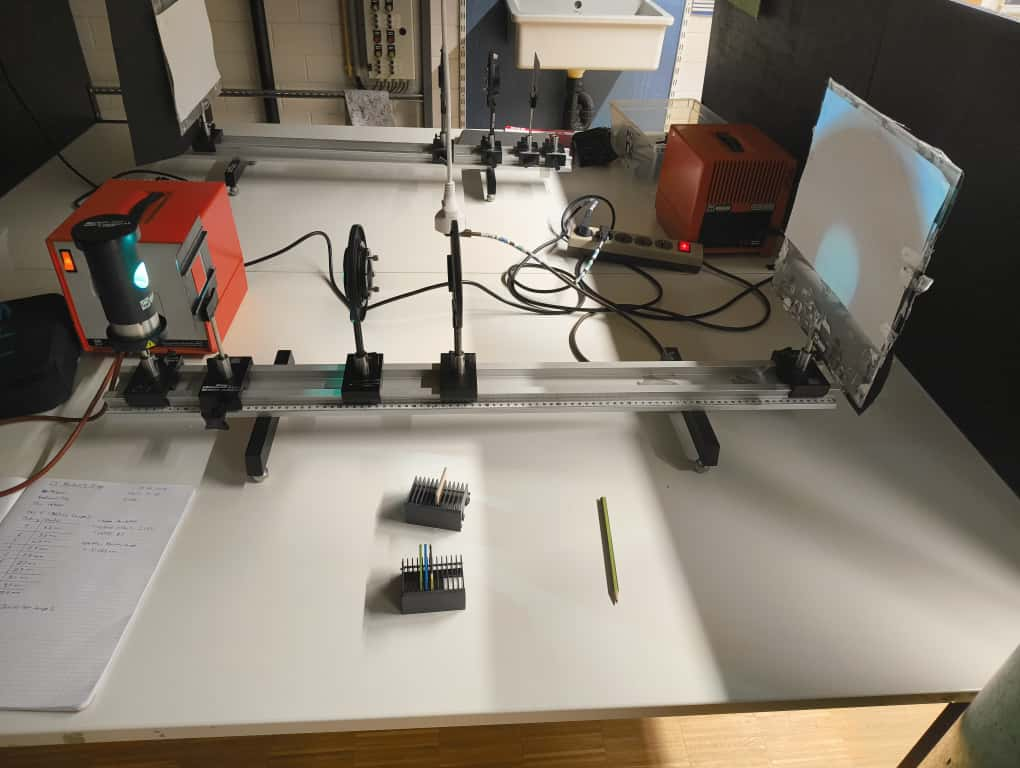
\includegraphics[width=0.9\linewidth]{Bilder/Versuchsaufbau O3.jpeg}
        \caption{Versuchsaufbau}
       \label{fig:SpASkizze}
\end{wrapfigure}
Bei dem zu betrachtenden Versuch, handelt es sich um einen simplen Versuchsaufbau auf einer 
Optischen Bank. Die zu verwendeten Bauteile sind folgende: Zwei lampen, einmal eine 
monochromatische Lampe wie zum beispiel eine Natriumdampf-Lampe und eine lampe mit einem 
breiten specktrum an sichtbaren Licht, wie zum beispiel eine Quecksilberdampf-Lampe, als 
nächstes Bauteil braucht man eine Blendenhalterung, das Newtonsche Farbglas welches aus 
einer Plan-konvexen Linse mit einem groszen krümmungsradius und einer sehr glatten 
Glasscheibe besteht, um Messdaten besser ablesen zu können ist auf der Glasscheibe zusätzlich 
noch eine skala aufgedruckt die den Maszstab veranschaulicht. Die letzten zwei Bauteile sind 
dazu da um besser die Interferenzmuster des Newton-Glases sehen zu können, das ist einmal 
eine Vergröszerungslinse und einen Schirm um das Muster auch abbilden zu können. %Bild vom versuchsaufbau


\subsection{Versuchsdurchführung}

Nun zur Versuchsdurchführung, der erste Schritt der Durchführung ist der Aufbau aller 
Bauteile auf der optischen bank, angefangen mit dem Schirm, der Vergröszerungslinse, dem 
Newtonschen-Glas, der Blendenhalterung und der Lichtquelle. Beim ersten Teil des Versuchs 
wird die Lampe mit mono chromatischen Licht verwendet. Sobald man nun die Lampe einschaltet 
und das Bild am Schirm scharf gestellt hat, kann man schon das Interferenzmuster Muster 
erkennen welches gemessen wird. Damit aber keine Ergebnisse verfälscht werden muss zuerst 
das Newtonsche-Farbglas richtig eingestellt werden. Hierzu werden die schrauben die, die 
Linse und die Glasplatte verbinden solange verstellt bis aus der Mitte des Bildes kein 
neuer Ring erscheint. Nun wird mithilfe der Skala auf der Glasplatte der Radius der dunklen 
Ringe ermittelt. Im zweiten Teil des Versuchs wird nun die monochromatische Lichtquelle mit 
einer Lichtquelle getauscht die mehrere Wellenlängen an Licht ausstrahlt. Sobald diese 
Lampe sich aufgeheizt hat wird der erste Teil des Versuchs wiederholt, da jetzt aber 
mehrere Wellenlängen von sichtbarem Licht ausgestrahlt werden wird vor dem messen ein 
Farbfilter in der Blendenhalterung befestigt. Dies wird jeweils für den Grünen-, Blauen- 
und Gelben- Farbfilter angewendet. 
\newpage
\section{Auswertung}
\newpage
\section{zusammenfassung}
\newpage
\section{Anhang}
\newpage
\section{Literaturverzeichnis}



\end{document}
